\documentclass[spanish,12pt, a4paper, twoside]{paper}

\let\oldsection\section
\def\section{\cleardoublepage\oldsection}

\usepackage{afterpage}

\newcommand\blankpage{%
    \null
    \thispagestyle{empty}%
    \addtocounter{page}{-1}%
    \newpage}

\usepackage[textwidth=15cm, textheight=22.5cm, top=3.5cm, bottom=3.5cm,left= 4cm,right=2cm]{geometry}
\usepackage[spanish]{babel}
\usepackage{xeCJK}
\setCJKmainfont{DroidSansFallbackFull.ttf}
%\usepackage[applemac]{inputenc} 
%POR DEFECTO SE ESTÁ USANDO EL PAQUETE PARA RECONOCER ACENTOS DE MAC, EN CASO DE USAR WINDOWS COMO SISTEMA OPERATIVO ELIMINAR LA LÍNEA ANTERIOR E INTRODUCIR LA SIGUIENTE
\usepackage[utf8]{inputenc}
\usepackage{libertine}

\usepackage{graphicx}
\usepackage{graphics}
\usepackage{amsmath,amssymb}
\usepackage{float}
\usepackage{changepage}
\usepackage{subcaption}
\usepackage{algorithm}
\usepackage{multirow}
\usepackage{hyperref}
\usepackage{listings}
\usepackage{xcolor}
\usepackage{wrapfig}
\usepackage{courier}
 
\definecolor{comment}{RGB}{0,128,0} % dark green
\definecolor{string}{RGB}{255,0,0}  % red
\definecolor{keyword}{RGB}{0,0,255} % blu
\definecolor{background}{RGB}{250,250,250}
 
\lstdefinestyle{mystyle}{
    commentstyle=\color{comment},
	stringstyle=\color{string},
	keywordstyle=\color{keyword},
	backgroundcolor=\color{background},
	basicstyle=\footnotesize\ttfamily,
	numbers=left,
	numberstyle=\tiny,
	numbersep=5pt,
	frame=lines,
	breaklines=true,
	prebreak=\raisebox{0ex}[0ex][0ex]{\ensuremath{\hookleftarrow}},
	showstringspaces=false,
	upquote=true,
    tabsize=2,
}

\lstdefinelanguage{JavaScript}{
  keywords={break, case, catch, continue, debugger, default, delete, do, else, false, finally, for, function, if, in, instanceof, new, null, return, switch, this, throw, true, try, typeof, var, void, while, with},
  morecomment=[l]{//},
  morecomment=[s]{/*}{*/},
  morestring=[b]',
  morestring=[b]",
  ndkeywords={class, export, boolean, throw, implements, import, this},
  keywordstyle=\color{keyword}\bfseries,
  ndkeywordstyle=\color{darkgray}\bfseries,
  identifierstyle=\color{black},
  commentstyle=\color{comment}\ttfamily,
  stringstyle=\color{string}\ttfamily,
  sensitive=true
}

\lstset{
   language=JavaScript,
   extendedchars=true,
   basicstyle=\ttfamily\footnotesize,
   showstringspaces=false,
   showspaces=false,
   numbers=left,
   numberstyle=\footnotesize,
   numbersep=9pt,
   tabsize=2,
   breaklines=true,
   showtabs=false,
   captionpos=b
}
 
\lstset{style=mystyle}

\begin{document}
%\maketitle
%\thispagestyle{empty}
\begin{titlepage}

\newcommand{\HRule}{\rule{\linewidth}{0.5mm}} % Defines a new command for the horizontal lines, change thickness here

\center % Center everything on the page
 
%	HEADING SECTIONS

\includegraphics[width=4cm]{recursos/logoEtsisi.png}
  \hspace{8cm}

\includegraphics[width=2cm]{recursos/logo.png}
\\[1cm]

\textsc{\Large Escuela Técnica Superior de Sistemas Informáticos}\\[0.5cm]
\textsc{\large Universidad Politécnica de Madrid}
\\[3cm]


%	TITLE SECTION
 \HRule \\[0.4cm]
{ \huge \bfseries BFMB: Framework Base para Bots Modulares}\\[0.4cm] % Title of your document
\HRule \\[2.5cm]

\textsc{\LARGE Trabajo Fin de Grado}\\[0.5cm] 
\textsc{\Large Grado en Ingeniería del Software }\\[2.5cm]

 %	AUTHOR SECTION
\begin{flushright}
\large
AUTOR: Ángel González Abad\\
TUTOR: Dr. Francisco Javier Gil Rubio
\end{flushright}

\vspace{1.3cm}

%	DATE SECTION
{{2019}}\\[3cm]
%	LOGO SECTION

\vfill % Fill the rest of the page with whitespace

\end{titlepage}

\afterpage{\blankpage}
\pagenumbering{roman}


%	AGRADECIMIENTOS
\section*{AGRADECIMIENTOS}
Aquí estarán los agradecimientos cuando se me ocurra que poner.

%	RESUMEN
\section*{RESUMEN}
Los chatbots no son aplicaciones que haya surgido recientemente, ya estuvieron presentes durante años en la investigación y en las redes con el desarrollo de Internet y la web. Pero es ahora cuando existe un ''boom'' en ellos, sobre todo gracias a los servicios que conforman la Web 2.0 y los recientes asistentes virtuales, tales como Siri, Alexa o Google Now.
\newline

El problema que surge a la hora de desarrollar un bot conversacional o una máquina de estados es cuando el desarrollador tiene como requisito la necesidad de interactuar con varios medios de forma simultánea. Por ejemplo, un sistema que requiera una comunicación simultánea entre redes sociales o un sistema que mande órdenes a un conjunto de dispositivos IoT (Internet of Things), ya que cada servicio utilizará protocolos e interfaces diferentes. Esto aumenta la complejidad en el desarrollo y puede producir duplicidades si se quieren desarrollar varios bots con usos diferentes.
\newline

Ante esta problemática, mi proyecto se basará en un sistema base para desarrollar bots (u otro tipo de automatismos software) multiprotocolo. Dicho sistema se compone de un servidor de comunicaciones central al que podemos anexar diferentes conectores que interactúan con los servicios de terceros. Cada conector pertenece a un servicio concreto, donde podremos activar los que nos sean útiles. La parte lógica del bot se comunica con el servidor a través de JSON-RPC sobre HTTP, HTTPS, TLS sobre TCP o TCP (dependiendo de las necesidades del proyecto).
\newline

La finalidad de este proyecto es hacer que el desarrollador se centre en la lógica y en la inteligencia que pueda tener en mayor o menor nivel en lugar de tener que centrarse en las interfaces de los servicios de terceros.


%	SUMMARY
\section*{SUMMARY}
Chatbots aren't recent applications, they were present during multiple years as reasearch projects and they were also present in the Internet during its growth. But now it's the moment where there's a ''boom'' in them, mainly caused by the Web 2.0 services and virtual assistants like Siri, Alexa or Google Now.
\newline

The problem begins when you want to develop a chatbot or a state machine where you need to interact with multiple sources simultaneously. For example, a system that requires a simultaneous communication between social networks or a system where you order some commands to a group of IoT (Internet of Things) devices, where each service will use different protocols and interfaces. These situations can increase the complexity in development process and can cause duplicities if you make multiple applications. 
\newline

Due to this problem, my project will be based in a base system for multiprotocol chatbot development (or another software automatisms). This system will be integrated by a central communication server where you can attach different connectors and the developer will activate some of them for his requisites. The logic part of the bot will communicate with the server using the JSON-RPC protocol over HTTP, HTTPS, TLS or TCP (according to the requirements of the project).
\newline

The purpose of this project is making the developers concentrate in his bot logic and functionality instead of thinking in the connections between his bot and external services.

%	ÍNDICE
\tableofcontents % indice de contenidos

%	INDICE DE FIGURAS Y TABLAS
\listoffigures
\listoftables

%	CAPÍTULOS DEL TRABAJO FIN DE MÁSTER
\newpage
\pagenumbering{arabic} 

\section{INTRODUCCIÓN Y OBJETIVOS}

Los chatbots no son aplicaciones que hayan surgido recientemente, sino que han tenido una larga historia por detrás. Desde el primer software chatbot (ELIZA en 1966), se han realizado desarrollos de chatbots hasta la actualidad. Pero es ahora cuando existe cierto surgir comercial de estos, gracias sobre todo a los asistentes virtuales de las grandes empresas tecnológicas como Siri \emph{(Apple)}, Alexa \emph{(Amazon)}, Watson \emph{(IBM)} o Google Assistant \emph{(Google)}.
\newline

Pero existe una problemática para quienes quieran realizar un chatbot: la necesidad de una conexión con el exterior para poder comunicarse. No suele ser compleja esta parte si solamente va a interactuar con un único servicio, pero cuando se requiere la conexión a múltiples servicios e interactuar con ellos de forma simultánea, la complejidad del desarrollo aumenta, llegando a dedicar más recursos a la conexión de servicios que a la lógica del software.
\newline

Para ello nace la idea propuesta para este proyecto final de grado. Me centraré en el desarrollo de un sistema base por el cual nuestro nuevo bot se conectará a los servicios que requiera. No solo valdría para chatbots y su conexión a redes de chat o redes sociales, sino también para máquinas de estados conectadas a servicios IoT. Este sistema se centra en las comunicaciones para que el desarrollador solamente tenga que centrarse en desarrollar la lógica, el cual ya supone bastante trabajo.
\newline

Este proyecto cubre los siguientes objetivos:

\begin{itemize}
\item El desarrollo de un servidor de comunicaciones que hará de mediador entre el bot y los servicios externos en Internet, usando para ello unos módulos denominados conectores.
\item La creación de uno o dos de esos módulos conectores para interactuar con los servicios de terceros.
\item La creación de un bot sencillo para poder realizar las demostraciones de funcionamiento.
\end{itemize}

\section{ESTADO DEL ARTE}

\subsection{Historia de los chatbots}

\subsubsection{Origen}

El origen del nombre ''chatbot'' viene de un software llamado CHATTERBOT, el cual era un jugador virtual del videojuego de mazmorras TinyMUD. La principal tarea de este bot era responder a las preguntas de los usuarios que tenían relación con la navegación por la mazmorra u objetos del juego. El mismo simulaba habilidad conversacional mediante reglas, mediante las cuales logró ''engañar'' a los usuarios y que estos creyeran que era un jugador humano más. \cite[pág. 2]{CANLI}

\subsubsection{ELIZA}
ELIZA fue un programa de procesamiento del lenguaje natural creado entre los años 1964 y 1966 por Joseph Weizenbaum (1923-2008) en el Laboratorio de Inteligencia Artificial del MIT (Instituto Tecnológico de Massachusetts). El objetivo de este software era demostrar la superficialidad de la comunicación entre humanos y máquinas.
\newline

El software que realizó fue una de las primeras vías de interacción entre persona y máquina mediante el uso del lenguaje natural. El mismo era una parodia de un terapéuta que ejercía psicoterapia centrada en el cliente, una teoría psicológica creada por el psicólogo norteamericano Carl Rogers. El software reutilizaba con frecuencia las frases enviadas por el cliente y las convertía en preguntas para el mismo.
\newline

ELIZA era un \emph{software} limitado, ya que solo fue programado para responder a ciertas palabras o frases clave. Así que lo normal era llegar a conversaciones sin sentido.

\subsubsection{ALICE}
ALICE (Artificial Linguistic Internet Computer Entity) es un bot con inspiraciones en ELIZA creado en 1995 por Richard Wallace. Puede procesar lenguaje natural mediante el uso de patrones. Dichos patrones se formaban con un lenguaje de marcado basado en XML llamado AIML. Actualmente, el lenguaje AIML sigue estando en desarrollo y la última versión disponible es la especificación 2.1, publicada en Marzo de 2018. 
\newline

A continuación os muestro un ejemplo de un patrón AIML:
\begin{lstlisting}[language=xml]
<?xml version="1.0" encoding="UTF-8"?>
   <aiml version="2.0">
     <category>
       <pattern>HI *</pattern>
       <template>Hello world!</template>
     </category>

     <category>
       <pattern>What is a chatbot</pattern>
       <template>
         A chatbot is a computer program designed to respond
         to text or voice inputs in natural language.
       </template>
     </category>
   </aiml>
\end{lstlisting}

\subsubsection{Siri (Apple)}

Siri es un asistente virtual desarrollado originalmente a principios de 2010 por una start-up del mismo nombre, la cual ofrecía dicha aplicación. Posteriormente fue adquirida por Apple para incorporarse como funcionalidad del sistema operativo iOS en Octubre de 2011 y se incorporó en el sistema MacOS Sierra, versión liberada en el año 2016.
\newline

Es capaz de reconocer el lenguaje natural mediante el uso de un conjunto de servidores remotos, es decir, no es el dispositivo en sí quien procesa la voz. Aparte, en base a ese procesamiento de voz, también procesa la orden para ser realizada por el dispositivo.
\newline

Además de reconocimiento del lenguaje natural mediante la voz, es capaz de expresar sus resultados con voz, lo que la otorga un valor añadido.
\newline

Por último, los desarrolladores de aplicaciones para iOS pueden añadir órdenes concretas para que puedan ser realizadas mediante la comunicación con Siri, usando la biblioteca SiriKit. SiriKit está disponible desde la versión 10 de iOS, la versión de macOS 10.12 y la versión 3.2 de watchOS (el sistema operativo que contienen los Apple Watch).

\subsubsection{Google Assistant}

Google Assistant es el asistente virtual desarrollado por Google, el cual es el núcleo de los productos Google Home pero también se encuentra presente en los dispositivos Android que incorporan las aplicaciones de Google (ya que hay dispositivos Android que no incluyen dichas aplicaciones).

\subsubsection{Alexa (Amazon)}

Alexa es el software que incorpora los dispositivos Echo de la misma empresa y puede integrarse en otros dispositivos como smartphones, ordenadores y otros dispositivos de terceros. Tiene las mismas funcionalidades que Google Assistant y Siri: permite la ejecución de órdenes o iniciar conversaciones en lenguaje natural y recibir respuestas al mismo nivel.

\subsection{Ejemplos de chatbots para usos posibles o reales.}

\subsubsection{Seguridad}

Como ejemplo de uso en el campo de la seguridad tenemos el chatbot Negobot. Desarrollado por la Universidad de Deusto en el año 2012, Negobot es un chatbot que simula ser un menor en los chats públicos de Internet para la detección de conductas pedófilas

\subsubsection{Sanidad}

Hablar sobre sistemas multiagente para detección de ETS.

\subsubsection{Banca}

\begin{wrapfigure}{r}{0.4\textwidth}
\centering
	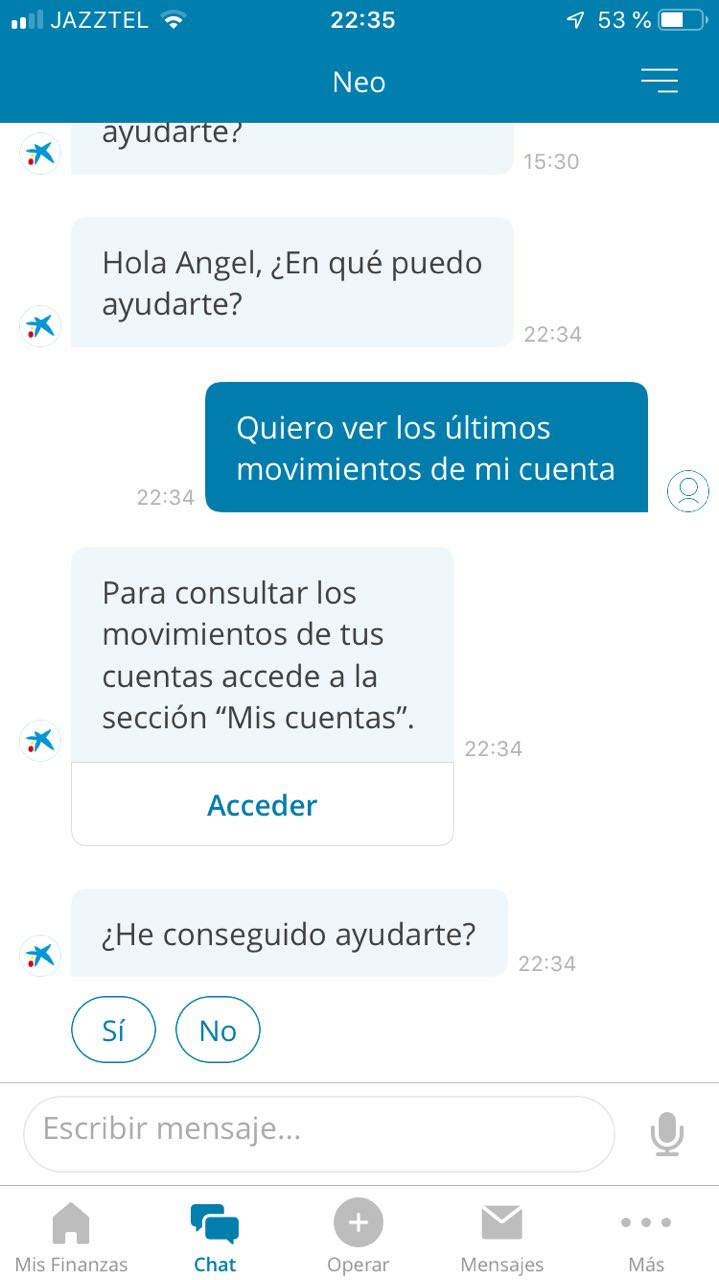
\includegraphics[width=0.4\textwidth]{recursos/neoCaixabank}
\caption{El chatbot Neo, desarrollado para la aplicación de gestión bancaria de Caixabank.}
\label{fig:Neo, bot de CaixaBank}
\end{wrapfigure}

Se están usando los chatbots en el ámbito de la banca para ser el sustituto de la sección de ayuda en las aplicaciones de gestión para el usuario, concretamente, de las secciones de \emph{Preguntas frecuentes} (o FAQ). Por ejemplo, está el caso de Neo, un chatbot que está incorporado en los servicios de \emph{Línea Abierta} (ahora \emph{CaixaBankNow}), del grupo CaixaBank.
\newline

El bot puede entender el lenguaje natural y responder a dichas preguntas. También incorpora un mecanismo de retroalimentación para mejorar el bot ante respuestas no válidas.

Este bot puede comunicarse con el usuario a través de la web de \emph{Línea Abierta}, la aplicación móvil de CaixaBank, Google Home y en Amazon Echo.

\subsection{Ética en los chatbots}

\section{ANÁLISIS}

\subsection{Idea base del proyecto}

La idea principal es el desarrollo de un sistema de comunicaciones con diversas APIs externas para facilitar el desarrollo de bots o automatismos que interactúen con ellos. En sí no forma una aplicación, sino que será una base para que otras personas puedan realizar sus aplicaciones. Por ello, es un framework.
\newline

Un framework es un software compuesto de componentes personalizables e intercambiables para el desarrollo de una aplicación. Podría considerarse como una aplicación genérica incompleta en donde se añadan las últimas piezas. \cite[pág. 1]{FrameworkJJG}

\subsection{Tecnologías usadas}

\subsubsection{JSON-RPC}

JSON-RPC es un protocolo de llamada a procedimiento remoto (Remote Procedure Call) cliente-servidor cuyos mensajes se componen de datos codificados en formato JSON (Javascript Object Notation). Es un protocolo agnóstico, puede realizar comunicaciones cliente-servidor a través de HTTP, HTTPS o TCP, entre otros. La especificación más reciente es la versión 2.0, publicada en 2010.

Como el protocolo usa JSON como mensaje, dispone de las mismas características que un fichero JSON: dispone de los cuatros tipos primitivos (String, Number, Boolean y Null) y de dos tipos de estructura (Object y Array).
El protocolo en sí se basa en dos modelos de datos: petición (Request) y respuesta (Response), los cuales explico a continuación:

\begin{itemize}
\item \textbf{Objeto petición (Request):} La llamada a procedimiento remoto en JSON-RPC se basa en enviar este objeto a un servidor, el cual dispone de los siguientes atributos:

\begin{itemize}
\item \textbf{jsonrpc:} Atributo que especifica la versión del protocolo JSON-RPC. Debe indicar el número de versión del protocolo. Es decir, si es la versión 2.0, debe ponerse "2.0".

\item \textbf{method:} Un String donde se indica el método a invocar. Cualquier nombre de método es válido excepto los que empiecen con "rpc.", ya que son de uso interno.

\item \textbf{params:} Un atributo de tipo estructura que indica los parámetros a enviar al método. Es un atributo que puede ser opcional.

\item \textbf{id:} Un identificador establecido por el cliente que puede ser un tipo distinto de Boolean (y Null, en base a las actualizaciones de la especificación). Si este valor no está includo, el protocolo considera la petición como una notificación.
\end{itemize}

\item \textbf{Objeto respuesta (Response):} La llamada a procedimiento remoto en JSON-RPC debe devolver una respuesta a cada petición excepto si es una notificación. El objeto respuesta tiene los siguientes atributos:

\begin{itemize}
\item \textbf{jsonrpc:} Atributo que especifica la versión del protocolo JSON-RPC. Debe indicar el número de versión del protocolo. Es decir, si es la versión 2.0, debe ponerse "2.0".

\item \textbf{result:} Este atributo es obligatorio si el resultado es exitoso y, en caso contrario (error), no debe estar presente. Siempre va a ser un atributo de estructura.

\item \textbf{error:} Este atributo debe existir en los casos de error y no aparecer en casos de éxito. Siempre va a ser un atributo de estructura.

\item \textbf{id:} El identificador en las respuestas es obligatorio y debe ser el mismo id que el recibido en el objeto de la petición. En caso de no llegar un id correcto, el valor de este atributo debe ser Null.
\end{itemize}

\item \textbf{Objeto error:} Si una llamada a procedimiento remoto encuentra un error, el objeto respuesta debe incorporar este objeto de error en el atributo denominado como tal. El objeto error tiene los siguientes atributos:

\begin{itemize}
\item \textbf{code:} Código de error de JSON-RPC

\item \textbf{message:} Un String que indica la descripción resumida del error.

\item \textbf{data:} Atributo de tipo primitivo o de estructura que entrega información adicional del error. Es un atributo opcional.
\end{itemize}

\end{itemize}

\subsection{Servicios utilizados}

\subsubsection{Tadoº}

Tadoº GmbH es una empresa tecnológica alemana con sede en Múnich y es un fabricante de sistemas de automatización de calefacción y refrigeración para el hogar conectados a Internet.
\newline

Fundado en el año 2011 por Johannes Schwarz, Christian Deilmann y Valentin Sawadski, el nombre de dicha compañía está inspirado en una unión de las expresiones japonesas ''tadaima'' (ただいま), que significa ''Estoy en casa'' y ''okaeri'' (おかえり), que significa ''Bienvenido'' a la hora de dirigirse a alguien con quien convives. 
Puede parecer que este detalle no aporta valor en este documento pero es lo contrario, ya que uno de los valores añadidos de sus sistemas de automatización es, precisamente, la gestión de la climatización basándose en la geolocalización.
\newline

Su gestión basada en geolocalización se realiza de la siguiente forma: El usuario o usuarios de la vivienda tienen asociado un dispositivo móvil, el cual debe tener la app de la compañía instalada y configurada. Esta app recoge la posición actual y se compara con un \emph{geofence} \footnote{El término \emph{geofence} es un perímetro virtual asociado a un área geográfica. Su utilidad se basa en la ejecución de eventos en software ante un suceso de entrada o salida del área definida. } definido por el usuario maestro de la vivienda. Cuando todos los usuarios de la vivienda abandonan la zona definida por el \emph{geofence}, Tado ordena la desconexión de la calefacción o la reducción de la temperatura de las estancias.
\newline

Otra de sus funcionalidades es la detección de ventanas abiertas. Los sensores instalados (termostatos y válvulas) detectan la temperatura y en la humedad, y los cambios repentinos en los mismos se asocian con la apertura de ventanas. Ante ello, Tado desconecta la calefacción por un tiempo definido en la configuración (entre 5 y 60 minutos) para evitar el consumo innecesario de energía. Esta funcionalidad es desactivable si no se precisa de ella (la estancia no tiene ventanas, por ejemplo).
\newline

La última funcionalidad adicional que provee es el ajuste de potencia en la calefacción basándose en el tiempo atmosférico actual. La calefacción se ajusta en base a la estimación de incidencia solar que puede haber.

\paragraph{Dispositivos}

Tadoº, en sus sistemas de calefacción, tiene distintos dispositivos de gestión, los cuales explico a continuación:

\begin{itemize}
\item\textbf{Puente de conexión (Bridge):} Es el dispositivo de conexión entre Internet (la api de Tado) y la red 6LoWPAN\footnote{6LoWPAN (IPv6 over Low-Power Wireless Personal Area Networks) es un estándar que adapta la transmisión de paquetes IPv6 a redes que siguen el estándar IEEE 802.15.4, los cuales son dispositivos con recursos muy limitados y un flujo de datos muy bajo. Otra característica de esta red es la capacidad de crear redes en malla.} en la que se comunican los dispositivos entre sí. Funciona con una conexión Ethernet y una conexión USB para alimentación eléctrica.

\item\textbf{Termostato:} Dispositivo que tiene la capacidad de encender o apagar la caldera o ajustar su potencia (según compatibilidad de calderas). Para ello, dispone de un relé para la conmutación. Incluye sensores para la medida de temperatura y humedad. Funcionan con tres pilas AAA y pueden ser instalados también como controladores de temperatura inalámbricos.

\item\textbf{Válvula termostática:} Mecanismo eléctrico que incluye sensores para la medición de temperatura y humedad. Con ellos, activa un motor que regula la apertura de la válvula del radiador donde se encuentre instalado y también pueden regularse de forma manual. Funcionan con dos pilas AA.
\end{itemize}

Pueden ver las fotografías de cada dispositivo en la figura ~\ref{fig:aparatos tado}.
\newline

\begin{figure}[htp]
\begin{subfigure}{0.5\textwidth}
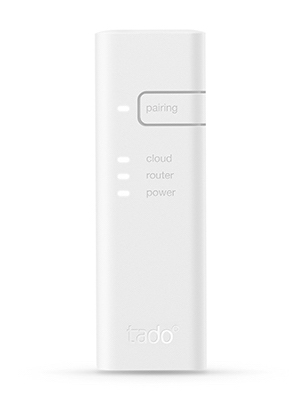
\includegraphics[width=\textwidth]{recursos/bridge.jpg}
\caption{Puente de conexión}
\label{fig:bridge tado}
\end{subfigure}
\begin{subfigure}{0.5\textwidth}
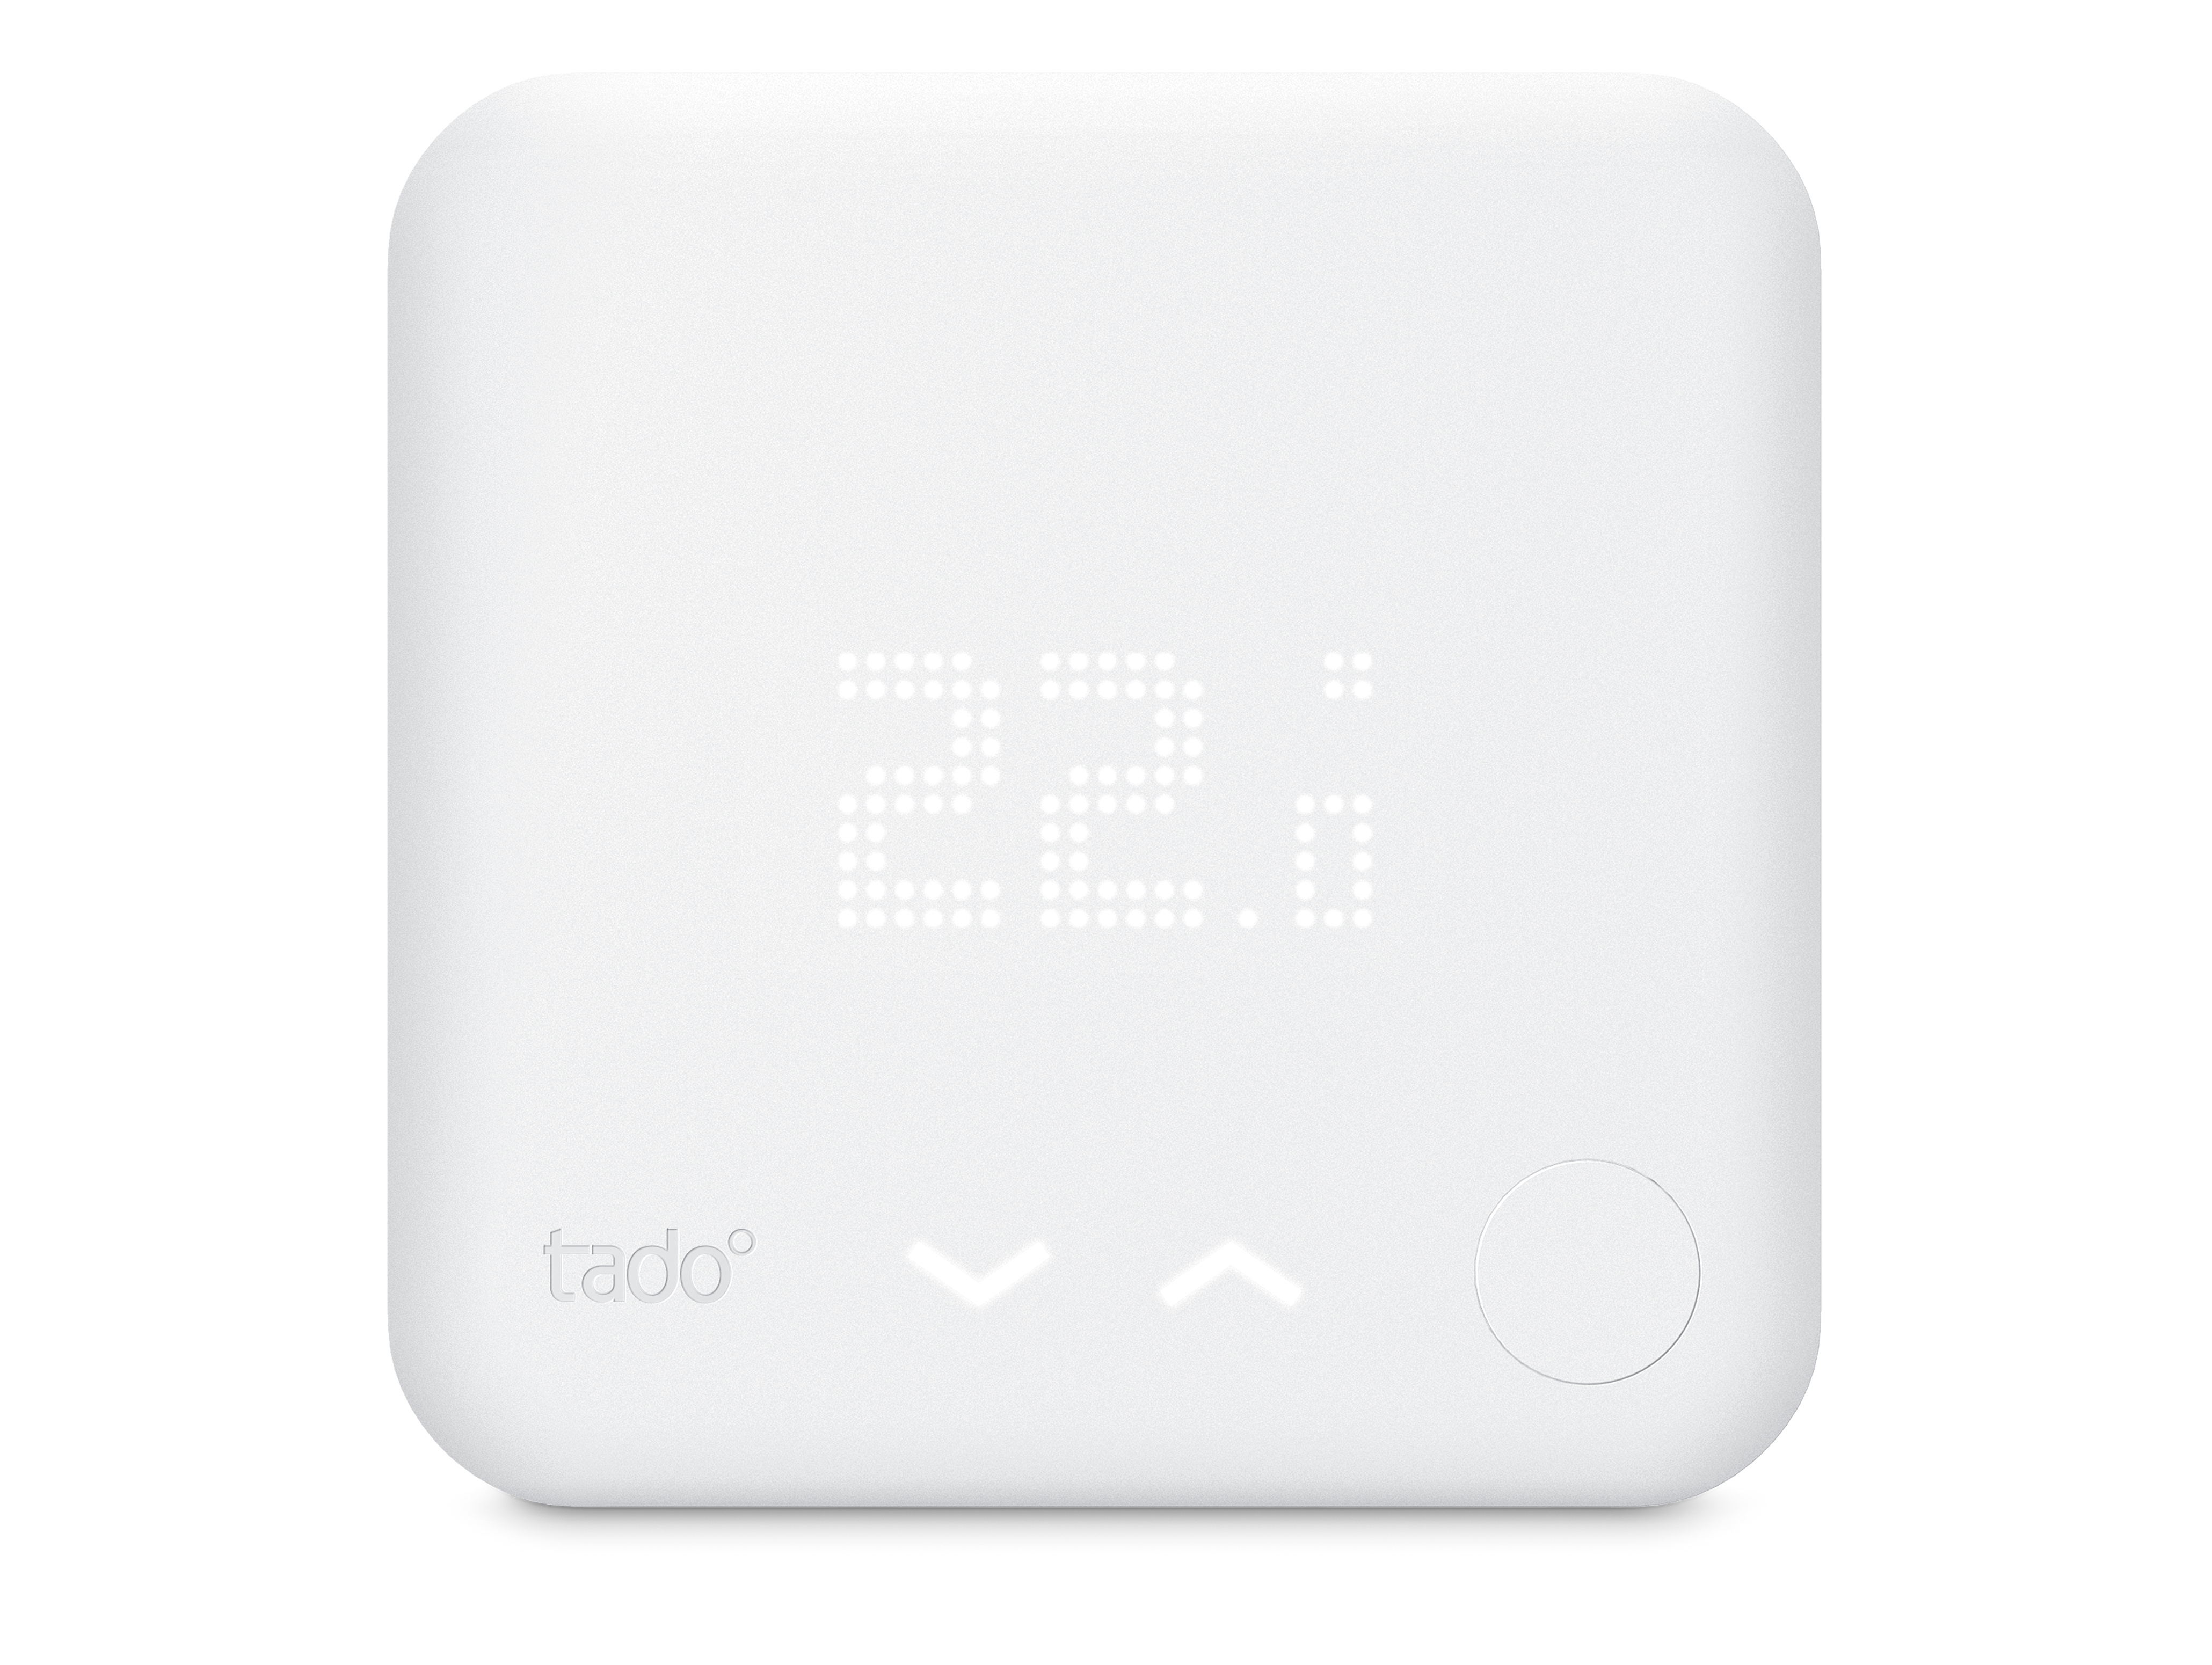
\includegraphics[width=\textwidth]{recursos/termostato.jpeg}
\caption{Termostato Tadoº}
\label{fig:termostato tado}
\end{subfigure}
\begin{subfigure}{0.5\textwidth}
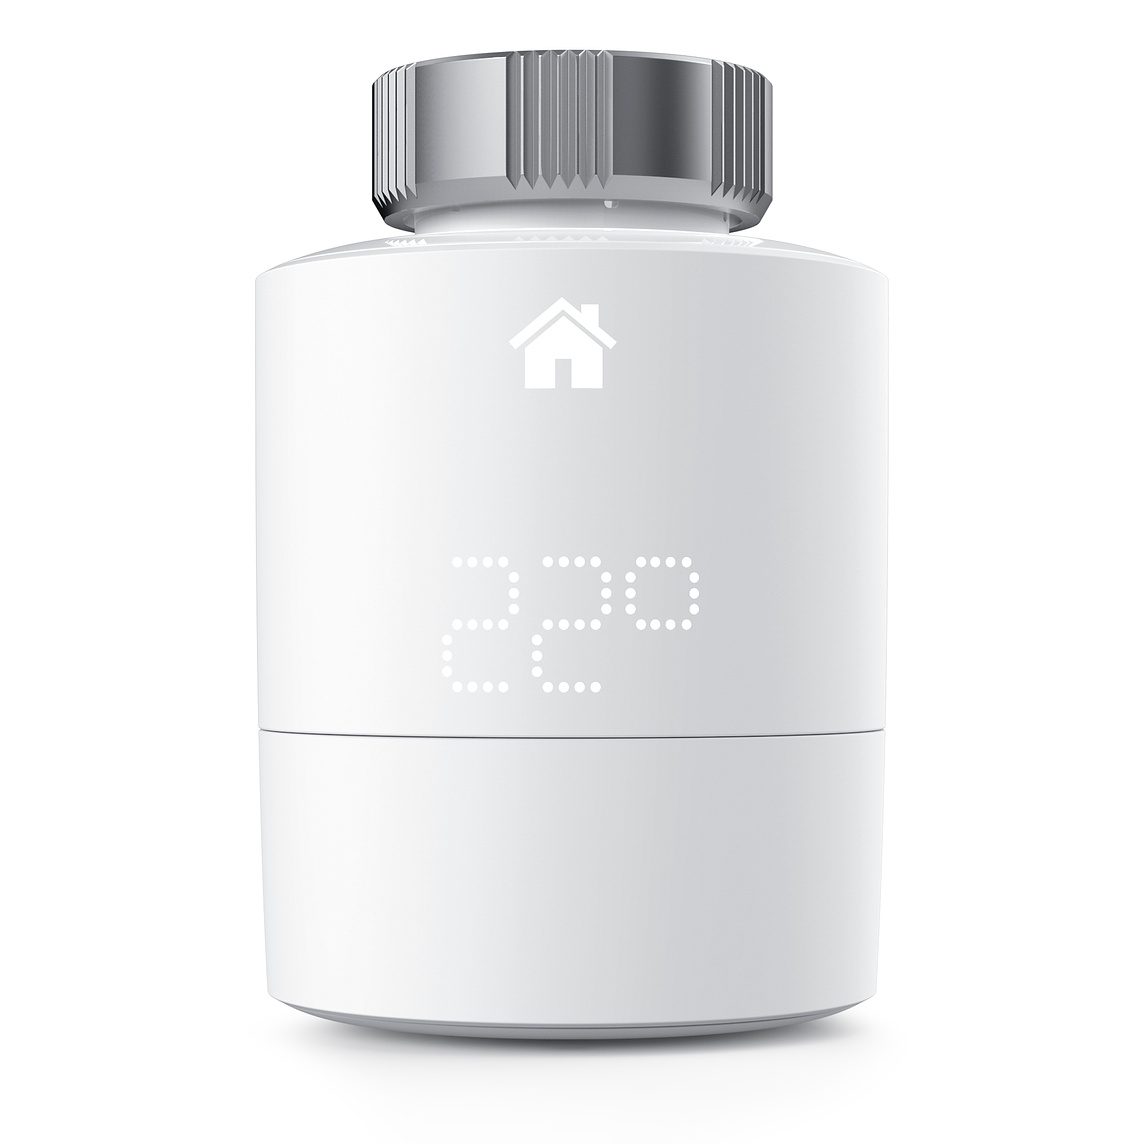
\includegraphics[width=\textwidth]{recursos/valvula.jpeg}
\caption{Válvula termostática Tadoº}
\label{fig:valvula tado}
\end{subfigure}

\caption{Aparatos de gestión de calefacción de la empresa Tadoº}
\label{fig:aparatos tado}
\end{figure}

También Tadoº tiene un dispositivo para gestionar de forma remota aparatos de aire acondicionado. Aun teniendo una forma diferente de trabajar a nivel técnico, dispone de las mismas funcionalidades que su equivalente en calefacción.

No entro en detalle en ese modelo de termostato porque queda fuera del proyecto (no dispongo de ese aparato y, por ello, no puedo probar su funcionamiento para adaptarlo al software que presento).

\subsubsection{Telegram}

Telegram es un servicio de mensajería instantánea y VoIP\footnote{VoIP: Voz por protocolo de Internet. Permite la transmisión de la voz a través de Internet usando el protocolo IP. Se usa actualmente por los proveedores de telefonía en lugar de la telefonía analógica.} creado en el año 2013 por Nikolai y Pavel Durov, quienes anteriormente crearon la red social VK, conocida sobre todo en la Federación de Rusia. Se estima que el servicio tiene 200 millones de usuarios activos al mes.

Las funcionalidades que dispone el servicio son las siguientes:

\begin{itemize}
\item \textbf{Acceso multiplataforma:} Telegram, a diferencia de otras redes, permite que un usuario esté activo en varios dispositivos a la vez, sin obligar a cerrar la sesión del resto de conexiones ni borrar el contenido de los chats almacenados. Lo que sí requiere es registrar la cuenta de Telegram con un número de teléfono móvil.

\item \textbf{Capacidad para adjuntos de gran tamaño:} Gracias al protocolo MTProto, creado por Nikolai Durov, es posible transferir adjuntos multimedia de hasta 1,5GB de tamaño.

\item \textbf{Grupos y canales:} Para conversaciones entre varias partes, existe la creación de grupos. En ellos pueden haber hasta 200 000 usuarios y se pueden realizar respuestas a un mensaje concreto del chat, mencionar a un usuario y generar \emph{hashtags}\footnote{Cadena de caracteres que se usa para clasificar la información presente. Sería un tipo de metadato.}. Dichos grupos pueden ser públicos o privados y disponer de varios administradores.

Por otra parte, los canales están pensados para difusión de mensajes por parte de uno o varios administradores. No existe límite de usuarios en los canales, por lo que cualquiera puede acceder. Al igual que los grupos, los canales pueden ser públicos o privados y tienen las mismas capacidades (pueden enviar adjuntos y mensajes, aunque el resto de usuarios no puedan hacer uso de ello).

\item \textbf{Bots:} En Telegram es posible el uso de bots y se incentiva el desarrollo de nuevos bots gracias a la documentación que se provee a los desarrolladores. Los bots pueden ser configurados de distintas formas (escuchando comandos, escuchando menciones o cualquier mensaje). También existen los \emph{inline bots}, son bots que no requiren estar presentes en un chat para funcionar y proveen datos en base una consulta.

\item \textbf{Stickers:} Una extensión de los emojis para poder expresar reacciones de forma breve y visual. Los stickers ya eran una característica que ya tenía la aplicación de mensajería LINE, creada en 2011.

\item \textbf{Chats secretos:} Telegram provee la opción de usar chats secretos entre dos usuarios. Para ello, se utiliza cifrado extremo a extremo\footnote{El cifrado extremo a extremo (End-to-end encryption) es un sistema de comunicación donde dos usuarios pueden comunicarse sin que sus mensajes sean captados por los nodos intermedios en una red.} Por defecto, Telegram no activa este tipo de chats, ya que ciertas funcionalidades de Telegram no funcionan con este tipo de chats, como el acceso multiplataforma o los bots.

\item \textbf{VoIP:} Al igual que otros servicios de mensajería actuales, dispone de servicio de llamadas por voz. 

\item \textbf{Inicio de sesión en sitios terceros:} Telegram también tiene implementado un sistema para poder iniciar sesión con las credenciales del servicio en páginas web terceras, siempre que estas incluyan los componentes necesarios para ello. 

\end{itemize}

\section{DISEÑO Y ARQUITECTURA DEL SISTEMA}

\subsection{Metodología de trabajo}

\textbf{PENDIENTE DE REALIZACIÓN}

\subsection{Casos de uso}

Los casos de uso para este proyecto están definidos a través de dos actores: el software que va a realizar las órdenes (el bot) y el usuario.

El bot realizará los siguientes casos de uso:

\begin{itemize}
\item El bot solicitará un autenticación con el servidor de comunicaciones (uno de los componentes del framework), el cual se envía un usuario y una contraseña al mismo. El servidor realiza la autenticación, comprobando si el usuario existe y si el hash de la contraseña guardada coincide con el hash generado de la contraseña enviada. Si la autenticación tiene éxito, se genera un token con los datos necesarios del usuario para poder realizar las acciones pertinentes.

\item El bot puede solicitar mensajes. Esta acción es una abstracción de las órdenes GET de una API HTTP REST. Para ello, antes de realizar acción alguna, se solicita el token que se recibió al autenticar para así validar la acción. Tras la verificación exitosa, se solicita los datos requeridos a través del servidor de comunicaciones. El servidor de comunicaciones dispone de unos componentes que denominaremos como "conectores", los cuales transforman la solicitud en los datos necesarios para el endpoint elegido. La respuesta o el error de la solicitud a la api la devuelve el servidor de comunicaciones.

\item El bot puede enviar mensajes. Esta acción es una abstracción de las órdenes POST, PUT y DELETE de una API HTTP REST. Al igual que con el caso de uso ya definido anteriormente, se verifica el token, se transforma el contenido y se envía a la api. La respuesta o error se devuelve a través del servidor de comunicaciones.
\end{itemize}

Por otra parte, el usuario realizará los siguientes casos de uso:

\begin{itemize}
\item A través de las aplicaciones que disponga cada servicio, el usuario interactúa con dichos servicios. Por ejemplo, puedo interactuar con el bot a través de un chat (Telegram) o cambiar la configuración de la calefacción (Tadoº).
\end{itemize}

Pueden ver el diagrama de casos de uso en la figura ~\ref{fig:Diagrama de casos de uso}.

\begin{figure*}
\centering
	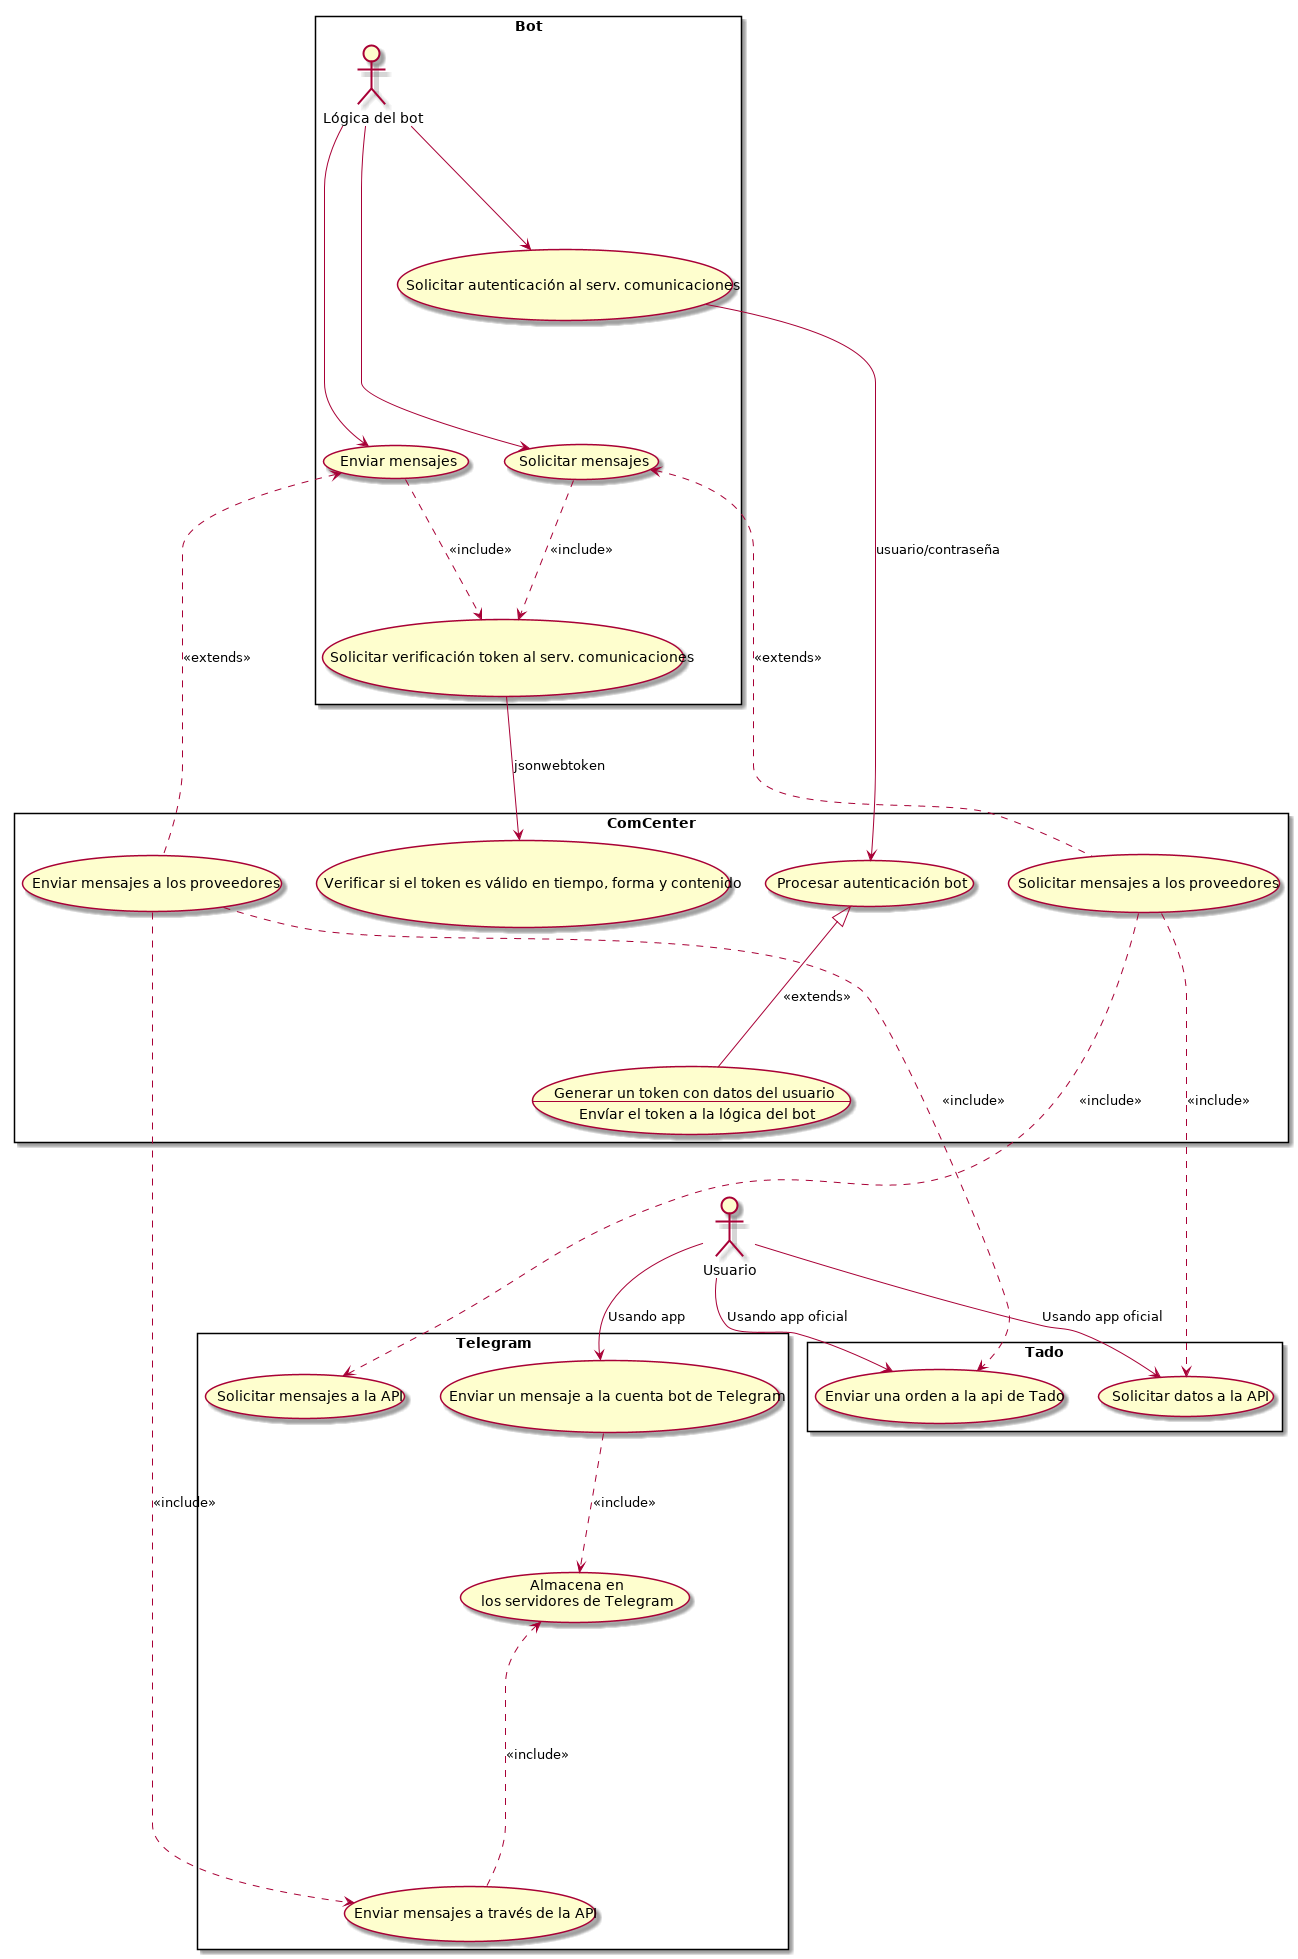
\includegraphics[width=\textwidth]{recursos/usecases}
\caption{Diagrama de casos de uso}
\label{fig:Diagrama de casos de uso}
\end{figure*}

\subsection{Infraestructura}

El framework BFMB requiere la ejecución de dos aplicaciones (el bot y el servidor de comunicaciones) y un servidor de Base de Datos (en este caso es MongoDB). Pueden ejecujarse en máquinas independientes o todo en una única máquina.
\newline

Ahora, vamos a definir en detalle cada aplicación:

\subsubsection{Software bot}

El software bot es la aplicación que realizará la persona que quiera utilizar este framework. Dicha aplicación puede desarrollarse en cualquier lenguaje de programación; el único requisito que debe tener para funcionar con este framework es la capacidad de poder usar el protocolo JSON-RPC, ya sea usando una biblioteca externa o una implementación propia.

\subsubsection{Servidor de comunicaciones}

El servidor de comunicaciones es una aplicación desarrollada en el lenguaje Typescript, el cual se compila a Javascript y se ejecuta usando NodeJS. Dicha aplicación contiene las siguientes funcionalidades:

\begin{itemize}
\item \textbf{Servidor JSON-RPC:} Usando una biblioteca externa llamada jayson, se ha realizado la implementación del servidor JSON-RPC. Lo único que hay que acoplar son los métodos que pueden ser accesibles a través del protocolo. Las aplicaciones bot pueden conectarse a través de protocolo TCP puro, TLS, HTTP o HTTPS. Para los protocolos seguros se requiere disponer de un certificado que pueda ser reconocido por una CA\footnote{Autoridad de certificación}, sea propia o externa.

\item \textbf{Conectores de servicio:} Los conectores son un elemento imprescindible para este software, son quienes permiten la conexión del servidor con los servicios externos a los que queramos acceder. Por el momento y para este proyecto, se han desarrollado dos conectores de servicio: uno para el servicio de mensajería instantánea Telegram y otro para un servicio que gestiona sistemas de calefacción IoT de la marca Tadoº. Son quienes realizan la conexión a la api usando los datos que se envían por parte del bot.

\item \textbf{Almacenamiento de credenciales:} Para garantizar que solo las aplicaciones autorizadas puedan usar el servidor de comunicaciones, se crean usuarios en una base de datos MongoDB. El detalle de los datos que se almacenan los mostraré en la siguiente sección pero, en resumen, el servidor almacena credenciales para acceder al servidor y los token y/o credenciales de las apis a las que debe acceder.
\end{itemize}

Pueden ver el diagrama de infraestructura en la figura ~\ref{fig:Infraestructura de nodos}.

\begin{figure*}
\centering
	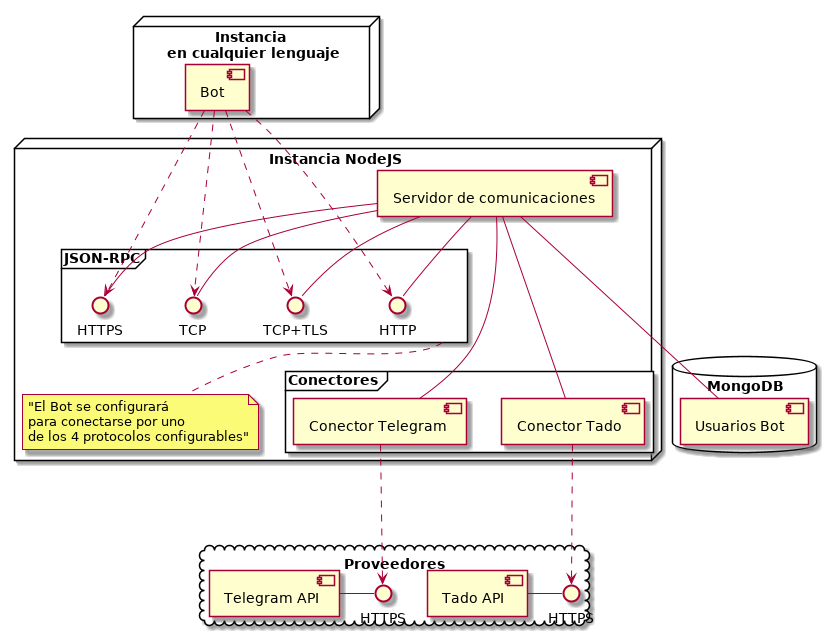
\includegraphics[width=\textwidth]{recursos/component}
\caption{Esquema de infraestructura (Diagrama de componentes)}
\label{fig:Infraestructura de nodos}
\end{figure*}

\subsection{Estructura de base de datos}

\begin{figure*}
\centering
	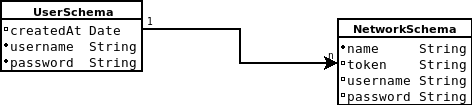
\includegraphics[width=0.65\textwidth]{recursos/schemes}
\caption{Estructura de base de datos}
\label{fig:Estructura de base de datos}
\end{figure*}

En la figura ~\ref{fig:Estructura de base de datos} pueden ver la sencilla estructura de base de datos que tenemos. Disponemos de dos entidades: usuario y red (UserSchema y NetworkSchema), las cuales vamos a detallar a continuación:

\begin{itemize}
\item\textbf{UserSchema:} Almacena los datos de acceso para el software se pueda conectar con nuestro servidor de comunicaciones. En ese modelo almacenaremos un nombre de usuario (\emph{username}), una contraseña (\emph{password}) y también almacenaremos la fecha de creación (\emph{createdAt}).

\item\textbf{NetworkSchema:} Almacena los datos necesarios para que el conector pueda conectarse con la api para la cual se ha realizado el desarrollo. Para ello almacenamos el nombre de la red (\emph{name}), el token (si el api funciona con un token permanente, como en la api de Telegram), el nombre de usuario (\emph{username}) y la contraseña (en los casos donde la autenticación se realiza por usuario y contraseña).
\end{itemize}

La relación que hay entre ambos es una relación \emph{1 a n}, donde para cada usuario (User) puede haber \emph{n} redes (Network).

\subsection{Disposición del código}

Por último, vamos a explicar la estructura de clases que existe en el framework que se ha desarrollado. Pueden ver el diagrama UML correspondiente en la figura ~\ref{fig:Diagrama de clases}.

Actualmente, este framework se compone de cuatro módulos:

\begin{itemize}
\item\textbf{bfmb-comcenter:} Es el paquete que conforma el servidor de comunicaciones.
\item\textbf{bfmb-base-connector:} Es el paquete que contiene una abstracción del conector, para así poder realizar llamadas a los conectores usando el polimorfismo\footnote{El polimorfismo es una relajación del sistema de tipos, de tal manera que una referencia a una clase acepta direcciones de objetos de dicha clase y de sus clases derivadas. \cite[Def. académica de Fernández, L.]{PgWebPolimorfismo}}.
\item\textbf{bfmb-telegram-connector:} Es el paquete que contiene el conector correspondiente para usar con la api de Telegram.
\item\textbf{bfmb-tado-connector:} El el paquete que contiene el conector correspondiente para usar con la api de Tadoº.
\end{itemize}

Los conectores adicionales seguirán el siguiente patrón como nombre:
\begin{center}bfmb-<SERVICIO>-connector\end{center}
Donde <SERVICIO> será el nombre de la api que corresponda.

Ahora nos centramos en cada módulo:

\subsubsection{bfmb-comcenter}

El módulo bfmb-comcenter, el servidor de comunicaciones, se compone de cinco clases, las cuales explicamos a continuación:

\begin{itemize}
\item\textbf{BFMBServer:} Es la clase maestra de este módulo y quien inicia el servidor JSON-RPC. Contiene una instancia de cada clase existente en el módulo y un atributo para acceder a la biblioteca jayson, la cual es la encargada de ejecutar el servidor JSON-RPC. También tiene implementado un patrón (o antipatrón si se abusa de su uso) singleton para poder obtener la instancia activa usando un método estático.
\item\textbf{MongoEvents:} Es la clase que contiene los métodos callback que se usan ante los eventos de la base de datos MongoDB. Con ello podemos continuar nuestro proceso si se ha logrado una conexión exitosa con la base de datos, mostrar un error en los casos no exitosos o cerrar la base de datos antes de finalizar la aplicación.
\item\textbf{AuthHandler:} Es la clase encargada de comprobar que las aplicaciones que se conecten con el servidor de comunicaciones tengan credenciales para ello. Comprueba la existencia de los usuarios en la base de datos y si la contraseña es válida. Tras ello, genera un token de acceso para que pueda validarse sin recurrir a sus credenciales originales por un tiempo definido.
\item\textbf{ConnectorManager:} Es la clase que contiene todos los conectores activos del servidor, donde se puede llamar al conector que corresponda a la api que solicitemos. Los conectores activos se inicializan en base a los datos de configuración, por lo que no varían en tiempo real.
\item\textbf{MessageHandler:}Es la clase encargada de procesar los mensajes que llegan al servidor de comunicaciones y ejecutar las acciones que soliciten. Normalmente esta clase busca el conector que corresponda con el servicio donde debe ejecutarse la orden y solicita la conexión que corresponde con su usuario, donde se la envía los datos para dicha api.
\end{itemize}

\subsubsection{bfmb-base-connector}

El módulo bfmb-base-connector es un módulo que contiene dos clases abstractas, cuyo objetivo es poder realizar polimorfismo entre las clases del servidor de comunicaciones y las clases de cada uno de los conectores de servicio. Se compone de dos clases:

\begin{itemize}
\item\textbf{Connector:} Es el gestor de la conexiones con la api que gestiona. Almacena n objetos conexión. Esta clase es abstracta y la usan los módulos conectores como clase padre en herencia.
\item\textbf{Connection:} Es la clase que define la conexión con la api. También es una clase abstracta, la cual usan los módulos conectores como clase padre. También sirve para poder realizar polimorfismo desde el servidor de comunicaciones.
\end{itemize}

\subsubsection{bfmb-telegram-connector y bfmb-tado-connector}

Los restantes módulos son los conectores con los que podremos conectarnos con las api de los distintos servicios en la red. Ambos módulos contienen como mínimo dos clases: conector (Connector) y conexión (Conection). Estos son clases hija de las clases Connector y Connection del módulo bfmb-base-connector.

\begin{figure*}
\centering
	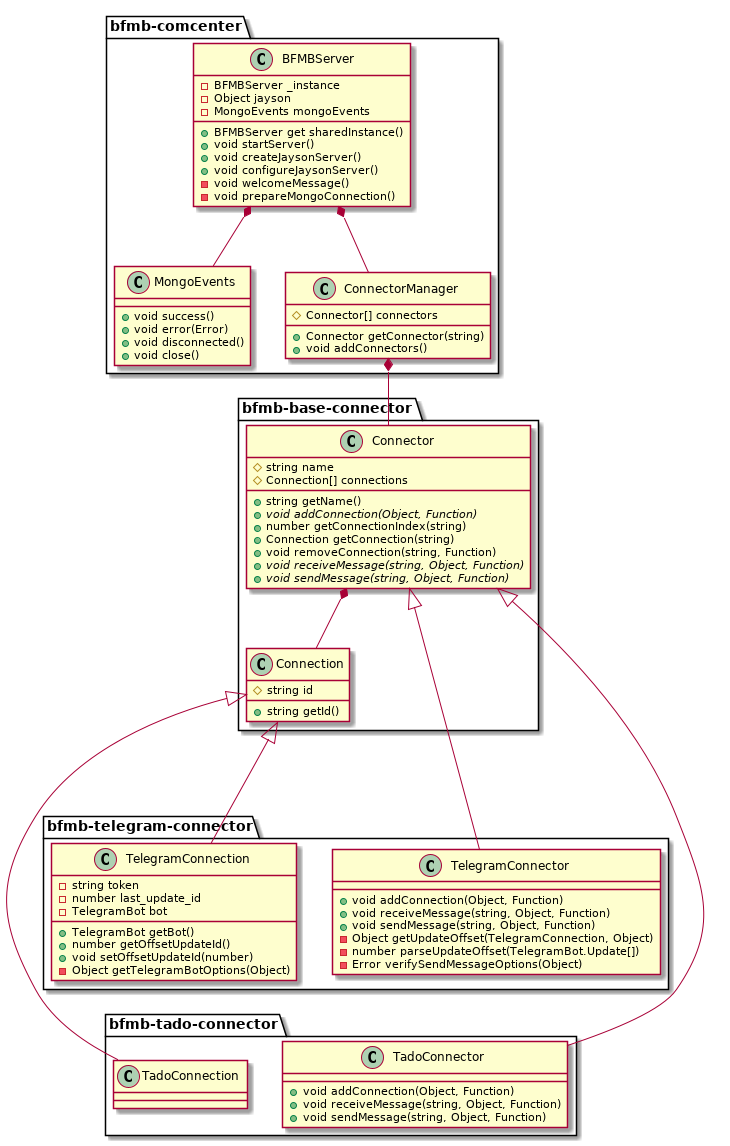
\includegraphics[width=\textwidth]{recursos/classes}
\caption{Diagrama de clases}
\label{fig:Diagrama de clases}
\end{figure*}

\section{DESARROLLO}

\subsection{Lenguaje usado en desarrollo}

El lenguaje usado para el desarrollo del software de este proyecto es Typescript, el cual vamos a hablar de él a continuación:

\subsubsection{Typescript}

Typescript es un lenguaje de programación que es un superconjunto de Javascript al que se le añade el tipado estático y la definición de objetos basados en clases. Es un proyecto de código abierto con licencia Apache 2.0 creado y mantenido por Microsoft.

\subsection{Dependencias}

\subsubsection{MongoDB}

MongoDB es un motor de base de datos orientado a documento. Se encuentra clasificado como una base de datos NoSQL, donde se usa una variante de JSON\footnote{Javascript Object Notation} como formato de documento.

\subsubsection{NodeJS}

NodeJS es un entorno de ejecución multiplataforma que permite ejecutar código escrito en Javascript fuera del entorno del navegador.

\subsubsection{Jayson}

Jayson es un módulo de NodeJS que se compone de un servidor y un cliente que cumplen con la especificación JSON-RPC 2.0, aunque también es compatible con la versión 1.0. Dispone de estas funcionalidades:

\begin{itemize}
\item Puede iniciar múltiples interfaces de red en el mismo proceso. Es decir, se puede iniciar un servidor que escuche el protocolo TCP y, a la vez, escuchar el protocolo HTTPS.
\item Soporta los protocolos TCP, HTTP y sus equivalentes seguros (TLS sobre TCP y HTTPS).
\item Permite el enrutamiento previo de métodos RPC. Por ejemplo, si tenemos una función que sume dos números y queremos hacer un método que añada dos a un valor numérico podremos utilizar el enrutamiento para llamar al método de suma en su lugar. Actualmente, mi proyecto no usa esta funcionalidad.
\item Dispone de un cliente que se puede ejecutar directamente desde la terminal / consola de comandos.
\end{itemize}

\subsubsection{Api de Telegram}

Telegram dispone de gran cantidad de documentación para la realización de bots para su servicio. Además, hay disponible varias bibliotecas para facilitar la tarea de desarrollo.

\subsubsection{Api de Tadoº}

En el caso de Tadoº, disponen de una api privada sin documentar, la cual usan las apicaciones desarrolladas por dicha empresa. Gracias a las labores de ingeniería inversa, se ha podido realizar el envío de comandos sin necesitar ninguna aplicación oficial. Esa labor ha abierto la puerta a realizar servicios adicionales especiales.

Por ejemplo, tenemos el proyecto tado-connect (\href{https://github.com/Martijn02/tado-connect}), donde configura los termostatos en modo ausente o presente en base a los usuarios conectados a una red wifi como alternativa a la geolocalización a través del smartphone.

\section{PRUEBAS}

\subsubsection{Mocha}

\section{MANUAL DE USUARIO}

\subsection{Instalación}

\subsubsection{Prerrequisitos}

Para poder trabajar con este framework se necesitan los siguientes requisitos software:

\begin{itemize}
\item Sistema operativo GNU/Linux (No puedo garantizar que funcione en otros sistemas operativos pero ningún requisito lo impide)
\item NodeJS (versión 8.16).
\item Base de datos MongoDB instalado o un acceso a un servidor con dicho motor de base de datos.
\item Conexión a Internet (necesario para interactuar con las apis disponibles).
\end{itemize}

\subsubsection{Procedimento de instalación}

Para poner en marcha el servidor de comunicaciones, primero comenzaremos con la instalación de los requisitos:

\paragraph{Instalación de NodeJS}

Para realizar la instalación de NodeJS puede optar por instalar el paquete que se encuentre en su distribución GNU/Linux o seguir el procedimiento de instalación del propio proyecto: \href{https://nodejs.org/es/download/package-manager/}{Instalando Node.js usando un gestor de paquetes}.
\newline

En el caso de Debian, la distribución GNU/Linux que he usado para el desarrollo, el procedimiento es el siguiente:

\begin{lstlisting}[language=sh]
# Using Debian, as root
curl -sL https://deb.nodesource.com/setup_8.x | bash -
apt-get install -y nodejs
\end{lstlisting}

El script provisto por Nodesource ya realiza todo lo necesario para instalar NodeJS.

\paragraph{Instalación de MongoDB} Para realizar la instalación de MongoDB se puede recurrir al paquete que se encuentre en el repositorio de su distribución. Eso sí, no está exento de inconvenientes porque ha habido un cambio de licencia en dicho software y esa nueva licencia (creada por la propia gente de MongoDB) genera conflicto con algunas distribuciones de GNU/Linux (SSPLv1)\footnote{Server Side Public License}.

En Debian Stretch y Jessie sigue disponible MongoDB, pero en Debian Buster (la futura versión estable) ya no se encuentra dicho paquete. Para ello toca seguir estos pasos:

\begin{enumerate}
\item Añadir los repositorios unstable de Debian. Hay que modificar el fichero /etc/apt/sources.list
\begin{lstlisting}[language=sh]
deb http://debian.redimadrid.es/debian/ buster main contrib non-free
deb-src http://debian.redimadrid.es/debian/ buster main

deb http://security.debian.org/debian-security buster/updates main
deb-src http://security.debian.org/debian-security buster/updates main

# Hay que añadir esta línea.
deb http://debian.redimadrid.es/debian/ unstable main contrib non-free
\end{lstlisting}

\item Después, hay que editar o crear el fichero mypreferences en /etc/apt/preferences.d/ y añadir el siguiente contenido:
\begin{lstlisting}[language=sh]
Package: *
Pin: release a=testing
Pin-Priority: 400

Package: *
Pin: release a=unstable
Pin-Priority: 300
\end{lstlisting}

Con esto hacemos que los paquetes que se encuentran en el repositorio testing (buster) tengan mayor prioridad que unstable. Así evitamos instalar paquetes de unstable más allá del propio MongoDB.

\item Por último, ejecutamos el comando apt de esta forma para instalar el paquete mongodb.
\begin{lstlisting}[language=sh]
sudo apt install -t unstable mongodb
\end{lstlisting}
\end{enumerate}

Este procedimiento no está exento de cambios y posiblemente acabe siendo anulado mientras pase el tiempo, ya que la última versión que mantendrá Debian será las que sean anteriores a mongo 4.0 (donde empieza el cambio de licencia). Tampoco está exento la posibilidad de cambios en el software para cambiar de motor de base de datos (véase: Líneas Futuras).

\paragraph{Instalación del servidor de comunicaciones}

Para realizar la instalación del servidor de comunicaciones debemos seguir estos pasos:

\begin{enumerate}
\item Primero debemos clonar el repositorio del servidor usando git. Si no está git instalado, en Debian basta con este comando:
\begin{lstlisting}[language=sh]
sudo apt install git
\end{lstlisting}

Después, realizamos la clonación:
\begin{lstlisting}[language=sh]
git clone https://github.com/BFMBFramework/ComCenter
\end{lstlisting}

\item Una vez obtenida la aplicación, tenemos que entrar en la carpeta raíz del proyecto e instalar las dependencias necesarias.
\begin{lstlisting}[language=sh]
cd ComCenter
npm install
\end{lstlisting}

\item Una vez realizado esto, ya tenemos instalado el servidor de comunicaciones. Actualmente, lo conectores vienen incluidos en el proceso de instalación de dependencias. No hace falta instalarlos aparte.
\end{enumerate}

\paragraph{Configuración del servidor de comunicaciones}

Para configurar el servidor de comunicaciones, disponen de una configuración de ejemplo en la carpeta raíz del software. Hagan una copia del mismo y editen el fichero.

\begin{lstlisting}[language=sh]
cp config-example.json config.json
nano config.json
\end{lstlisting}

Ahora explicamos qué opciones están disponibles en la configuración:
\begin{lstlisting}[language=Javascript]
{
	"db": {
		"url": "mongodb://localhost/comcenter",
		"encKey": "yfbmTM8/lZAH8H6PkGTcyK0H1bMk4kl0ovwq1xhX75w=",
		"signKey": "q8N6L+Lo345JsnUlSow4sPlKzo+XRJPYjT2Uq7mhlOkSi5kFkX0UoIY3etfm4UxtNHaM8xaX2HtkAhV7Gye0KA=="
	},
	"tokenConfig": {
		"secret": "W]5!>v$@NV!bgk8T?{$vP~o'^9P}S1",
		"algorithm": "HS512",
		"expiresIn": "24h"
	},
	"servers": [
		{
			"type": "tcp",
			"port": 3000
		},
		{
			"type": "http",
			"port": 3001
		},
		{
			"type": "https",
			"port": 3002,
			"cert": "/home/angel/certificados/certi.pem",
			"key": "/home/angel/certificados/certikey.key"
		},
		{
			"type": "tls",
			"port": 3003
		}
	],
	"modules": [
		"telegram",
		"tado"
	]
}
\end{lstlisting}

\begin{itemize}
\item\textbf{db:} Es el objeto donde definimos la configuración de base de datos.
\begin{itemize}
\item\textbf{db.url:} En este campo se introduce la url de conexión con la base de datos de MongoDB.

\item\textbf{db.encKey:} La base de datos se encuentra cifrada. Para ello, se necesita una pareja de claves para realizar el cifrado con estas. En este campo se almacena una clave de cifrado de 32 bytes en formato base64 (clave de 256bits).

\item\textbf{db.signKey:} En este campo se introduce la clave de firma de la base de datos. Se requiere que sea una clave de bytes en formato base64 (clave de 512 bits).

Para generar ambas claves se puede usar openssl de la siguiente forma:
\begin{lstlisting}[language=sh]
openssl rand -base64 32; openssl rand -base64 64;

yZ4dEBn2RILEOGA04kg6oIJHsm6QO4kcbT2jnjAaFTo= # Clave de cifrado
7n24rUz8G8KKojMo3LhUBvv2TUBW7LQPg+FkyzFtAPSaF3NimFBPhNgWM9s4n5fX
251ZD20BTd24OTKSmBSxNQ== # Clave de firma
\end{lstlisting}
\end{itemize}

\item\textbf{tokenConfig:} Es el objeto donde definimos la configuración de los tokens que generará el servidor de comunicaciones.

\begin{itemize}
\item\textbf{tokenConfig.secret:} En este campo introducimos el secreto que usará jsonwebtoken para generar los tokens con firma. El formato es un string y acepta carácteres alfanuméricos y símbolos.

\item\textbf{tokenConfig.algorithm:} En este campo indicaremos el algoritmo de firma a usar para la generación de los tokens. Por el momento se ha probado con algoritmos simétricos (HMAC con hash SHA), los cuales son:
\begin{itemize}
\item\textbf{none:} El token no se firma con ningún algoritmo.
\item\textbf{HS256:} El token se firmará con el algoritmo HMAC con hashing SHA256
\item\textbf{HS384:} El token se firmará con el algoritmo HMAC con hashing SHA384
\item\textbf{HS512:} El token se firmará con el algoritmo HMAC con hashing SHA512
\end{itemize}

\emph{En el futuro se definirán atributos para los algoritmos de firma asimétricos, ya que estos requieren clave privada y clave pública.}

\item\textbf{tokenConfig.expiresIn:} Campo en el que definimos la duración de los tokens generados. 

Si introducimos un valor numérico (no string), se considerará el tiempo de vida en segundos. 

Si introducimos un string con el valor numérico seguido de un carácter que pueda reconocerse como una unidad de tiempo (h, m, d, s, ms), se configurará el tiempo de vida del token en base a esa unidad. Por ejemplo, "24h" serían 24 horas y "7d" serían 7 días. 

En caso que el string solo tenga carácteres numéricos, se expresará como milisegundos.
\end{itemize}

\item\textbf{servers:} Servers es un array en el cual indicamos los servidores JSON-RPC que tendremos operativos, los cuales se configuran de la siguiente forma.
\begin{itemize}
\item\textbf{type:} En este campo indicamos el protocolo con el que levantaremos el servidor. Puede configurar los siguientes tipos:
\begin{itemize}
\item\textbf{tcp:} Servidor JSON-RPC usando el protocolo TCP.
\item\textbf{http:} Servidor JSON-RPC usando el protocolo HTTP.
\item\textbf{tls:} Servidor JSON-RPC usando el protocolo TLS.
\item\textbf{https:} Servidor JSON-RPC usando el protocolo HTTPS.
\end{itemize}

\item\textbf{port:} Puerto por el que escuchará este servidor.
\item\textbf{cert:} \emph{(Requerido cuando type es tls o https, ignorado en otros casos)} Ruta de acceso al fichero del certificado que vayamos a usar para securizar la conexiones a este servidor.
\item\textbf{key:} \emph{(Requerido cuando type es tls o https, ignorado en otros casos)} Ruta de acceso al fichero con la clave privada del certificado que hayamos seleccionado.

\emph{En caso de no encontrar el fichero cert y el fichero key en las rutas indicadas (o la omisión de los mismos) impedirá el funcionamiento de los servidores con protocolo tls o https y, por ello, no se iniciarán.}
\end{itemize}

\item\textbf{modules:} En este array indicaremos los módulos que arrancaremos de BFMBFramework, es decir, los conectores a las apis que necesitemos. Para ello, hay que introducir un string con el nombre del servicio.

Es decir, si queremos iniciar el conector bfmb-telegram-connector, debemos introducir Telegram. Si queremos iniciar el conector bfmb-tado-connector, debemos introducir "Tado" (y así con el resto).
\end{itemize}

\subsubsection{Inicio del servidor} Una vez que tengamos el servidor configurado, podremos iniciarlo con este comando. Desde la carpeta raíz del servidor:
\begin{lstlisting}[language=sh]
./bin/comcenter
\end{lstlisting}

Esta sería la salida esperada:
\begin{lstlisting}[language=sh]
info: Using configuration file from: /home/angel/Proyectos/PFG/ComCenter/config.json
info: Welcome to BFMB ComCenter 0.5.0
info: Connecting to MongoDB...
info: Connected to MongoDB database
info: Attaching connectors to Connector Manager
info: Raising tcp server on port 3000
info: Raising http server on port 3001
info: Raising https server on port 3002
error: Can't raise https server. No certificates.
info: Raising tls server on port 3003
error: Can't raise tls server. No certificates.
node-telegram-bot-api deprecated Automatic enabling of cancellation of promises is deprecated.
In the future, you will have to enable it yourself.
See https://github.com/yagop/node-telegram-bot-api/issues/319. module.js:653:30
\end{lstlisting}

Como pueden ver, si no se encuentran los certificados que se buscan, saltará un error en los logs para indicar que no se han podido iniciar los servidores tls y https configurados pero no detendrá la aplicación.

\subsection{Añadir usuarios al servidor de comunicaciones}

Para añadir usuarios al servidor, como no tenemos ningúna aplicación de administrador por el momento, tengo hecho un script en lenguaje Javascript que añade los usuarios que queramos.

\begin{lstlisting}[language=Javascript]
var mongoose = require('mongoose');
var config = require('../../config.json');
var User = require('../../dist/schemas/user').User;
var Network = require('../../dist/schemas/network').Network;

mongoose.connect(config.db.url, {useNewUrlParser: true});

if (!process.env.TG_TOKEN) throw new Error("No Telegram token defined.");
if (!process.env.TADO_USERNAME) throw new Error("No Tado login data defined.");
if (!process.env.TADO_PASSWORD) throw new Error("No Tado login data defined.");

var test = new User({
	username: 'TEST',
	password: 'test'
});

test.save(function (err) {
	if (err) throw err;

	var tgNetwork = new Network({
		name: 'Telegram',
		token: process.env.TG_TOKEN
	});

	tgNetwork.save(function (err) {
		if (err) throw err;
		console.log("Added Telegram network");
	});

	var tadoNetwork = new Network({
		name: 'Tado',
		username: process.env.TADO_USERNAME,
		password: process.env.TADO_PASSWORD
	});

	tadoNetwork.save(function (err) {
		if (err) throw err;
		console.log("Added Tado Network");
	})

	test.networks.push(tgNetwork);
	test.networks.push(tadoNetwork);
	test.save(function (err) {
		if (err) throw err;
		console.log("Added test user.");
	});
});
\end{lstlisting}

Para añadir el usuario con username 'TEST' y password 'test' basta con ejecutar el script de esta forma.

\begin{lstlisting}[language=sh]
TG_TOKEN=<token de bot Telegram> TADO_USERNAME=<usuario de Tadoº> TADO_PASSWORD=<contraseña de Tadoº> nodejs ./add-mocha-user.js
\end{lstlisting}

Para cambiar el username y el password a añadir basta con editar las líneas 13 y 14 del script. No es la mejor forma de configurar usuarios y en el futuro se implementará una aplicación de gestión con el fin de facilitar esta tarea.

\subsection{Cómo interactuar con el servidor de comunicaciones}

Como se puede ver en la figura ~\ref{fig:Comunicación entre sistemas}, nuestro automatismo se conecta únicamente con el servidor de comunicaciones usando para ello el protocolo JSON-RPC, por lo que se puede realizar el bot o automatismo con cualquier lenguaje que tenga un cliente de dicho protocolo.

\begin{figure*}
\centering
	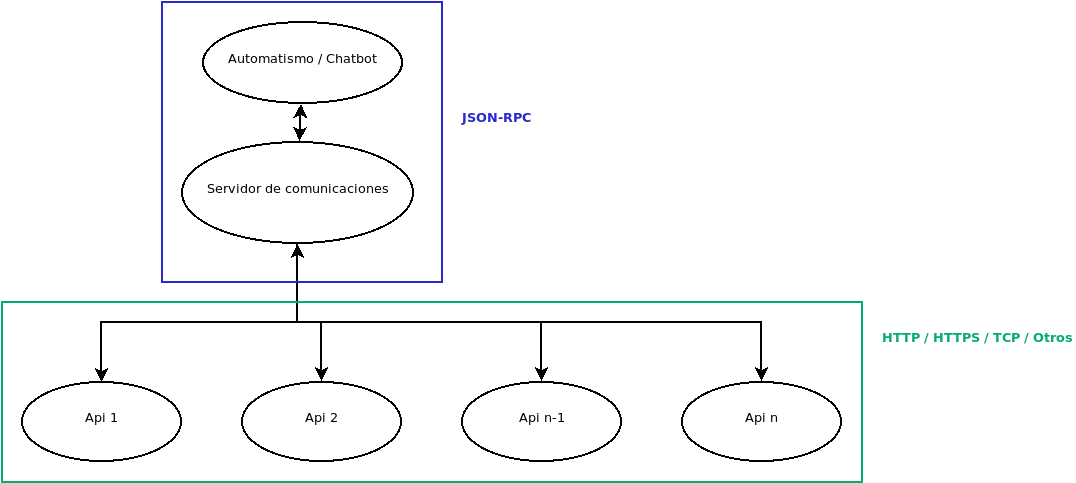
\includegraphics[width=\textwidth]{recursos/Comunication}
\caption{Comunicación entre sistemas}
\label{fig:Comunicación entre sistemas}
\end{figure*}

Para los ejemplos en código, voy a usar Typescript y usaré el cliente jayson.

\subsubsection{Realizar login en el servidor}

Para poder comunicarse con el servidor, es necesario iniciar sesión en él. Para ello, hay que ejecutar el comando RPC 'authenticate' pasando como opciones el username y el password del usuario del servidor.

\begin{lstlisting}[language=Javascript]
this.jayson.request('authenticate',
 { username: 'username', password: 'password' },
 function(err: Error, response: any) {
			if (err) { 
				// Caso error
			} else {
				// Caso éxito
			}
		});
\end{lstlisting}

\subsubsection{Obtener información del usuario de la api}

Para obtener los datos del usuario de la api que se quisiese acceder, basta con mandar el comando RPC 'getMe'. Como opciones es necesario el token que habremos recibido tras realizar la autenticación con el comando anterior, la red a la que queremos enviar esta orden (recuerde que debe empezar en mayúscula) y las opciones para dicha red (en este caso será un objeto vacío).

\begin{lstlisting}[language=Javascript]
this.jayson.request('getMe',
 {token: 'token srv comunicaciones', network: 'Mired', options: {}}, 
 function(err: Error, response: any) {
   if (err) {
     // Caso error
   } else {
     // Caso éxito
   }
});
\end{lstlisting}

\subsubsection{Comando de recepción de información}

Para realizar una llamada que equivaldría al método HTTP GET, usamos el comando RPC 'receiveMessage'. Como opciones es necesario el token recibido al autenticarse en el servidor de comunicaciones, también hay que indicar la red a la que vamos enviar el comando. Por último, las opciones forman parte de los parámetros necesarios para solicitar la recepción de datos. Por ejemplo, el conector Tadoº necesita las opciones \emph{api\_method} y \emph{home\_id}. Si no se enviase algún parámetro obligatorio, el error que devolviese el comando lo indicará.

\begin{lstlisting}[language=Javascript]
this.jayson.request('receiveMessage',
 {token: 'token srv comunicaciones', network: 'Mired',
 options: {api_method: 'getZones', home_id: 'home_id'}}, 
 function(err: Error, response: any) {
 
 });
\end{lstlisting}

\subsubsection{Comando de envío de información}

Para realizar una llamada que equivaldría a los métodos POST, PUT y DELETE de HTTP, usamos el comando RPC 'sendMessage'. Como opciones también necesitamos el token recibido (al igual que en los otros métodos), también es necesario indicar la red a la que vamos a enviar el comando. Pôr último, las opciones forman parte de los parámetros necesarios para solicitar el envío de información. Por ejemplo, en el caso de usar el conector de Tadoº, es necesario usar los parámetreos \emph{api\_method} y \emph{home\_id}. También en este caso, si no se llegase a enviar un parámetro que fuese obligatorio, el error devuelto lo indicará.

\begin{lstlisting}[language=Javascript]
this.jayson.request('sendMessage',
 {token: 'token srv comunicaciones', network: 'Mired',
 options: {api_method: 'setZoneOverlay', home_id: 'home_id'}}, 
 function(err: Error, response: any) {
 
 });
\end{lstlisting}
 
\section{CONCLUSIONES}

\textbf{PENDIENTE DE REALIZACIÓN}

\section{LÍNEAS FUTURAS}

Tras el desarrollo actual y los resultados dados, se puede ver que hay distintas líneas futuras a partir de ahora. Algunas de ellas son mejoras del software para permitir una mayor portabilidad y otras pertenecen a posibles desarrollos adicionales.

\begin{itemize}
\item Cambiar el motor de base de datos usado en el servidor de comunicaciones. 

Actualmente se usa MongoDB por conveniencia en el desarrollo de este proyecto (el uso de la biblioteca mongoose ayudó mucho), pero sería más apropiado usar bases de datos portables como SQLite o NeDB  y evitar la instalación de un servidor adicional para el poco volumen de información que tiene que almacenar, aunque eso conlleve la modificación de parte del código fuente para pasar de un motor de base de datos a otro.

Otro motivo para abrir esta línea de desarrollo es el cambio de licencia de MongoDB en su versión más reciente (4.0). Eso está generando rechazo en la comunidad del software libre y la comunidad opensource, llegando al punto que ciertas distribuciones GNU/Linux (Fedora y Debian) estén eliminando o planteando que se elimine este software de sus repositorios. \cite{MongoDBLicense} \cite{MongoDBRemoveRequest}

\item Incorporar un gestor web de usuarios para el servidor de comunicaciones.

Actualmente, se están añadiendo los usuarios y configuraciones a través de un script. La incorporación de un gestor web serviría para facilitar la configuración del mencionado servidor. Se podría plantear incluso desarrollar el gestor como una aplicación por comandos independiente del software servidor.

\item Acoplar un motor de reconocimiento de lenguaje natural para la parte bot.

Ahora mismo, el bot realizado para este proyecto no procesa lenguaje natural, sino que se basa en comandos para la realización de órdenes. Se podría incorporar una implementación de ELIZA con un script personalizado para estos casos de uso. En lugar de un script psicoterapeuta, uno que reconozca frases del estilo ''Pon la cocina a 23ºC'' y lo asocie con la orden que debe ejecutar. Se tardaría menos en realizar esto que crear un motor IA desde cero.

\item Cambiar la abstracción del servidor de comunicaciones a métodos de api REST (Crear, consultar, editar y eliminar). Sería la equivalencia a las acciones HTTP POST, GET, PUT y DELETE en lugar de tener una abstracción de dos métodos (\emph{receive} y \emph{send}).

\item Implementación de un contenedor Docker que permita la implantación de este sistema sin la necesidad de enfocar los esfuerzos en lograr el entorno de trabajo adecuado para el sistema en donde se quiera instalar.
\end{itemize}

\section*{ANEXOS}


%	REFERENCIAS
\newpage

\begin{thebibliography}{00}
\bibitem{CANLI} \textsc{Pérez-Diaz, D.} y \textsc{Pascual-Nieto, I.},
	\textit{Conversational Agents and Natural Language Interaction: Techniques and Effective Practices}, IGI Global, 2011 ISBN: 9781609606183
	
\bibitem{PCBEvolution} \textsc{Cerdas Mendez, D.}
	\textit{Historia de los chatbots y asistentes virtuales}, Planeta Chatbot, \url{https://planetachatbot.com/evolucion-de-los-chatbots-48ff7d670201}, [Visitado el 4/3/2019]
	
\bibitem{WeizenbaumNYT} \textsc{Markoff, J.}
	\textit{Joseph Weizenbaum, Famed Programmer, Is Dead at 85}, The New York Times, \url{https://www.nytimes.com/2008/03/13/world/europe/13weizenbaum.html}, [Visitado el 12/3/2019]
	
\bibitem{SCPhillipsTadoIEng} \textsc{Phillips, S.}
	\textit{The Tado API v2}, SCPhillips.com, \url{http://blog.scphillips.com/posts/2017/01/the-tado-api-v2/}, [Visitado el 12/3/2019]
	
\bibitem{JSONRPC} \textsc{JSON-RPC Working Group} \textit{JSON-RPC version 2.0 specification}, \url{https://www.jsonrpc.org/specification}, [Visitado el 8/4/2019]

\bibitem{CleanTechTado} \textsc{Cleantech investor} \textit{Tadoº raises \texteuro10m from Target Partners and Shortcut Ventures}, \url{https://web.archive.org/web/20140821174647/http://www.cleantechinvestor.com/portal/mainmenucomp/companiest/3258-tado/11706-tado-raises.html}, [Visitado el 17/4/2019]

\bibitem{TadoDeviceSpecs} \textsc{Tado GmbH} \textit{Technical documentation of Tado}, \url{http://www.free-instruction-manuals.com/pdf/pa_1184164.pdf}, [Visitado el 19/4/2019]

\bibitem{Tado6LoWPAN} \textsc{Jiménez Ruiz, L.} \textit{Diseño e implementación de etapa de comunicación basada en 6LoWPAN para plataforma modular de redes de sensores inalámbricas}, Archivo documental de la UPM, 2016, \url{http://oa.upm.es/43013/1/TFG_LUIS_JIMENEZ_RUIZ.pdf}, [Visitado el 19/4/2019]

\bibitem{TelegramFAQ} \textsc{Telegram} \textit{Telegram FAQ}, \url{https://telegram.org/faq}, [Visitado el 19/4/2019]

\bibitem{TelegramLogin} \textsc{Telegram} \textit{Telegram Login for Websites}, \url{https://telegram.org/blog/login}, [Visitado el 19/4/2019]

\bibitem{FrameworkJJG} \textsc{J. Gutiérrez, J.} \textit{¿Qué es un framework web?}, \url{http://www.lsi.us.es/~javierj/investigacion_ficheros/Framework.pdf}, [Visitado el 5/5/2019]

\bibitem{PgWebPolimorfismo} \textsc{Álvarez, M.Á.} \textit{Polimorfismo en Programación Orientada a Objetos}, \url{https://desarrolloweb.com/articulos/polimorfismo-programacion-orientada-objetos-concepto.html}, [Visitado el 12/5/2019]

\bibitem{Jayson} \textsc{Lundgren, T. y otros} \textit{Jayson is a simple but featureful JSON-RPC 2.0/1.0 client and server for node.js}, \url{https://github.com/tedeh/jayson/blob/master/README.md}, [Visitado el 8/5/2019]

\bibitem{MongoDBLicense} \textsc{MuyLinux} \textit{MongoDB pincha en hueso: nadie acepta su nueva licencia}, \url{https://www.muylinux.com/2019/01/17/mongodb-rechazo-nueva-licencia/}, [Visitado el 12/5/2019]

\bibitem{NodeSourceDebian} \textsc{Nodesource} \textit{README de distributions en GitHub}, \url{https://github.com/nodesource/distributions/blob/master/README.md#deb}, [Visitado el 12/5/2019]

\bibitem{MongoDBRemoveRequest} \textsc{Debian Bug Reports} \textit{\#916107 - mongodb: MongoDB should not be part of a stable release}, \url{https://bugs.debian.org/cgi-bin/bugreport.cgi?bug=916107}, [Visitado el 15/5/2019]

\bibitem{NeDB} \textsc{Louis Chatriot} \textit{NeDB: The JavaScript Database, for Node.js, nw.js, electron and the browser}, \url{https://github.com/louischatriot/nedb}, [Visitado el 21/5/19]

\bibitem{NeoCaixabank} \textsc{Caixabank} \textit{Web Neo \textbar Banca Digital \textbar CaixaBank}, \url{https://www.caixabank.es/particular/banca-digital/web-neo.html?loce=sh-part-Neo-5-terrat-BancaDigital-WebCaixabanknow-NA}, [Visitado el 22/5/19]

\bibitem{AIMLFoundation} \textsc{AIML Foundation} \textit{AIML Foundation}, \url{http://www.aiml.foundation}, [Visitado el 27/5/19]

\bibitem{SiriAppleMain} \textsc{Apple Support} \textit{Use Siri on all your Apple devices}, \url{https://support.apple.com/en-us/HT204389}, [Visitado el 1/6/19]

\bibitem{SiriKit} \textsc{Apple Developer} \textit{SiriKit}, \url{https://developer.apple.com/sirikit/}, [Visitado el 1/6/19]

\bibitem{SiriHistory} \textsc{Bianca Bosker} \textit{SIRI RISING: The inside story of Siri's origins - And why she could overshadow the iPhone - Huffpost}, \url{https://www.huffingtonpost.com/2013/01/22/siri-do-engine-apple-iphone_n_2499165.html}, [Visitado el 1/6/19]

\bibitem{GoogleAssistant} \textsc{Google} \textit{El Asistente de Google \textbar Tu Google personalizado}, \url{https://assistant.google.com/intl/es_es/}, [Visitado el 3/6/19]

\bibitem{AmazonAlexa} \textsc{Amazon} \textit{Amazon Alexa}, \url{https://developer.amazon.com/es/alexa}, [Visitado el 3/6/19]

\bibitem{ChemaAlonsoNegobot} \textsc{Chema Alonso (El lado del mal)} \textit{Un informático en el lado del mal: NegoBot: Una bot para detectar pedófilos en chats}, \url{http://www.elladodelmal.com/2013/07/negobot-una-bot-para-detectar-pedofilos.html}, [Visitado el 4/6/19]

\bibitem{DeustoNegobot} \textsc{Laorden, C., Galán, P. y otros} \textit{Negobot: Agente conversacional basado en teoría de juegos para la detección de conductas pedófilas.}, \url{http://paginaspersonales.deusto.es/claorden/publications/2012/Negobot.pdf}, [Visitado el 4/6/19]
\end{thebibliography}
\end{document}

